\documentclass[border=6pt]{standalone}
\usepackage{tikz}
\usetikzlibrary{arrows.meta,positioning,calc,shapes.geometric,fit,backgrounds,patterns,matrix,decorations.pathreplacing}
\begin{document}
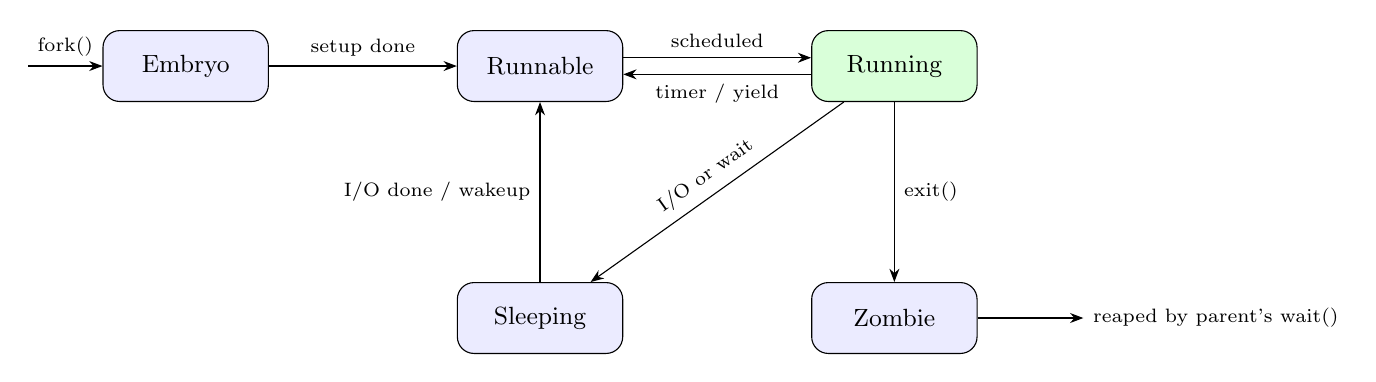
\begin{tikzpicture}[>=Stealth,font=\small]
\tikzstyle{st}=[draw,rounded corners=6pt,minimum width=2.1cm,minimum height=0.9cm,fill=blue!8]
\node[st] (emb) at (0,0) {Embryo};
\node[st] (run) at (4.5,0) {Runnable};
\node[st,fill=green!15] (rng) at (9,0) {Running};
\node[st] (zom) at (9,-3.2) {Zombie};
\node[st] (slp) at (4.5,-3.2) {Sleeping};
\draw[->] (-2,0) -- node[above]{\scriptsize fork()} (emb);
\draw[->] (emb) -- node[above]{\scriptsize setup done} (run);
\draw[->,transform canvas={yshift=3pt}] (run) -- node[above]{\scriptsize scheduled} (rng);
\draw[->,transform canvas={yshift=-3pt}] (rng) -- node[below]{\scriptsize timer / yield} (run);
\draw[->] (rng) -- node[right]{\scriptsize exit()} (zom);
\draw[->] (rng) -- node[above,sloped]{\scriptsize I/O or wait} (slp);
\draw[->] (slp) -- node[left]{\scriptsize I/O done / wakeup} (run);
\draw[->] (zom) -- ++(2.4,0) node[right]{\scriptsize reaped by parent's wait()};
\end{tikzpicture}
\end{document}
